% **************************************************
% Tesis Doctoral: Desarrollo de vehículos a base de arabinoxilanos para la liberación controlada de metformina
% Programa: Doctorado en Ciencias de los Alimentos y Salud Humana
% Institución: Universidad Autónoma del Estado de Hidalgo
% Editor: Nombre del estudiante de posgrado
% **************************************************

% **************************************************
% Definición de documento:
% **************************************************
\documentclass[letterpaper,twoside,openright,final]{book}
\usepackage{AleXandra}
\usepackage{AbsResPhDThesis}
\usepackage[object=vectorian]{pgfornament}
\usetikzlibrary{calc}

% **************************************************
%	Configuración del idioma:
% **************************************************
\usepackage[utf8]{inputenc}
\usepackage[english, spanish, es-tabla]{babel}
\selectlanguage{spanish}

% **************************************************
%	Paquetes:
% **************************************************
\usepackage{amsmath,amsthm,amsfonts,amssymb,gensymb,textcomp}
\usepackage{graphicx} % Insertar figuras, [demo]
\usepackage{subfig} % Insertar subfiguras
\usepackage{psfrag,layout,listings}
\usepackage{listings}
\usepackage{tikz}
\usepackage{xifthen}
\usepackage[skins]{tcolorbox} %Insertar cajas.
\usepackage{marvosym} %Insertar símbolos de contacto.
\usepackage[Glenn]{fncychap} %Options: Sonny, Lenny, Glenn, Conny, Rejne, Bjarne, Bjornstrup
\usepackage[final]{pdfpages} %Configuración de PDF Externos

\usepackage{makeidx} % Índice alfabético
\usepackage[printonlyused,withpage]{acronym} % Crear lista de acrónimos.
\usepackage[refpages]{gloss} %Configuración de glosario
\usepackage{appendix} %Configuración de anexos
\usepackage[authoryear]{natbib} %orden establecido en el argumento
\usepackage{apalike}

\usepackage{multicol} % utilizar texto en columnas
\setlength{\columnseprule}{0.2pt}

\spanishdecimal{.} %Cambia las comas por puntos en los números


% **************************************************
%	Formato de hipervínculos:
% **************************************************
\usepackage{hyperref}
\hypersetup{
	colorlinks=true,
	citecolor=iColor006,
	filecolor=iColor006,
	linkcolor=iColor006,
	urlcolor=iColor006,
	bookmarksopen=true,
	pdfpagelayout=TwoPageRight,
	pdftitle={Development arabinoxylans devices for controlled release of metformin},
	pdfauthor={Jesús Guadalupe P. Flores},
	pdfsubject={PhD Thesis JGPFlores},
	pdfproducer={LaTeX},
	pdfkeywords={Feruloylated arabinoxylans, Hydrogels, Metformin}
}

% **************************************************
%	Formato de contadores de secciones y subsecciones:
% **************************************************
\makeatletter
\renewcommand\@seccntformat[1]{\color{iColor001!80} {\csname the#1\endcsname}\hspace{0.5em}}
\makeatother

\graphicspath{{pictures/}} % Localizacion de las figuras

\makegloss % Crear glosario
\makeindex % Crear índice

% **************************************************
% Comienza la escritura del documento:
% **************************************************
\begin{document}

% **************************************************
\frontmatter % --- InicioDocumento
% **************************************************
\pagestyle{empty} %Quita los números de las primeras páginas
% --- Insertar PDFs: \includepdf[pages=inicial-final]{nombre_del_documento}
	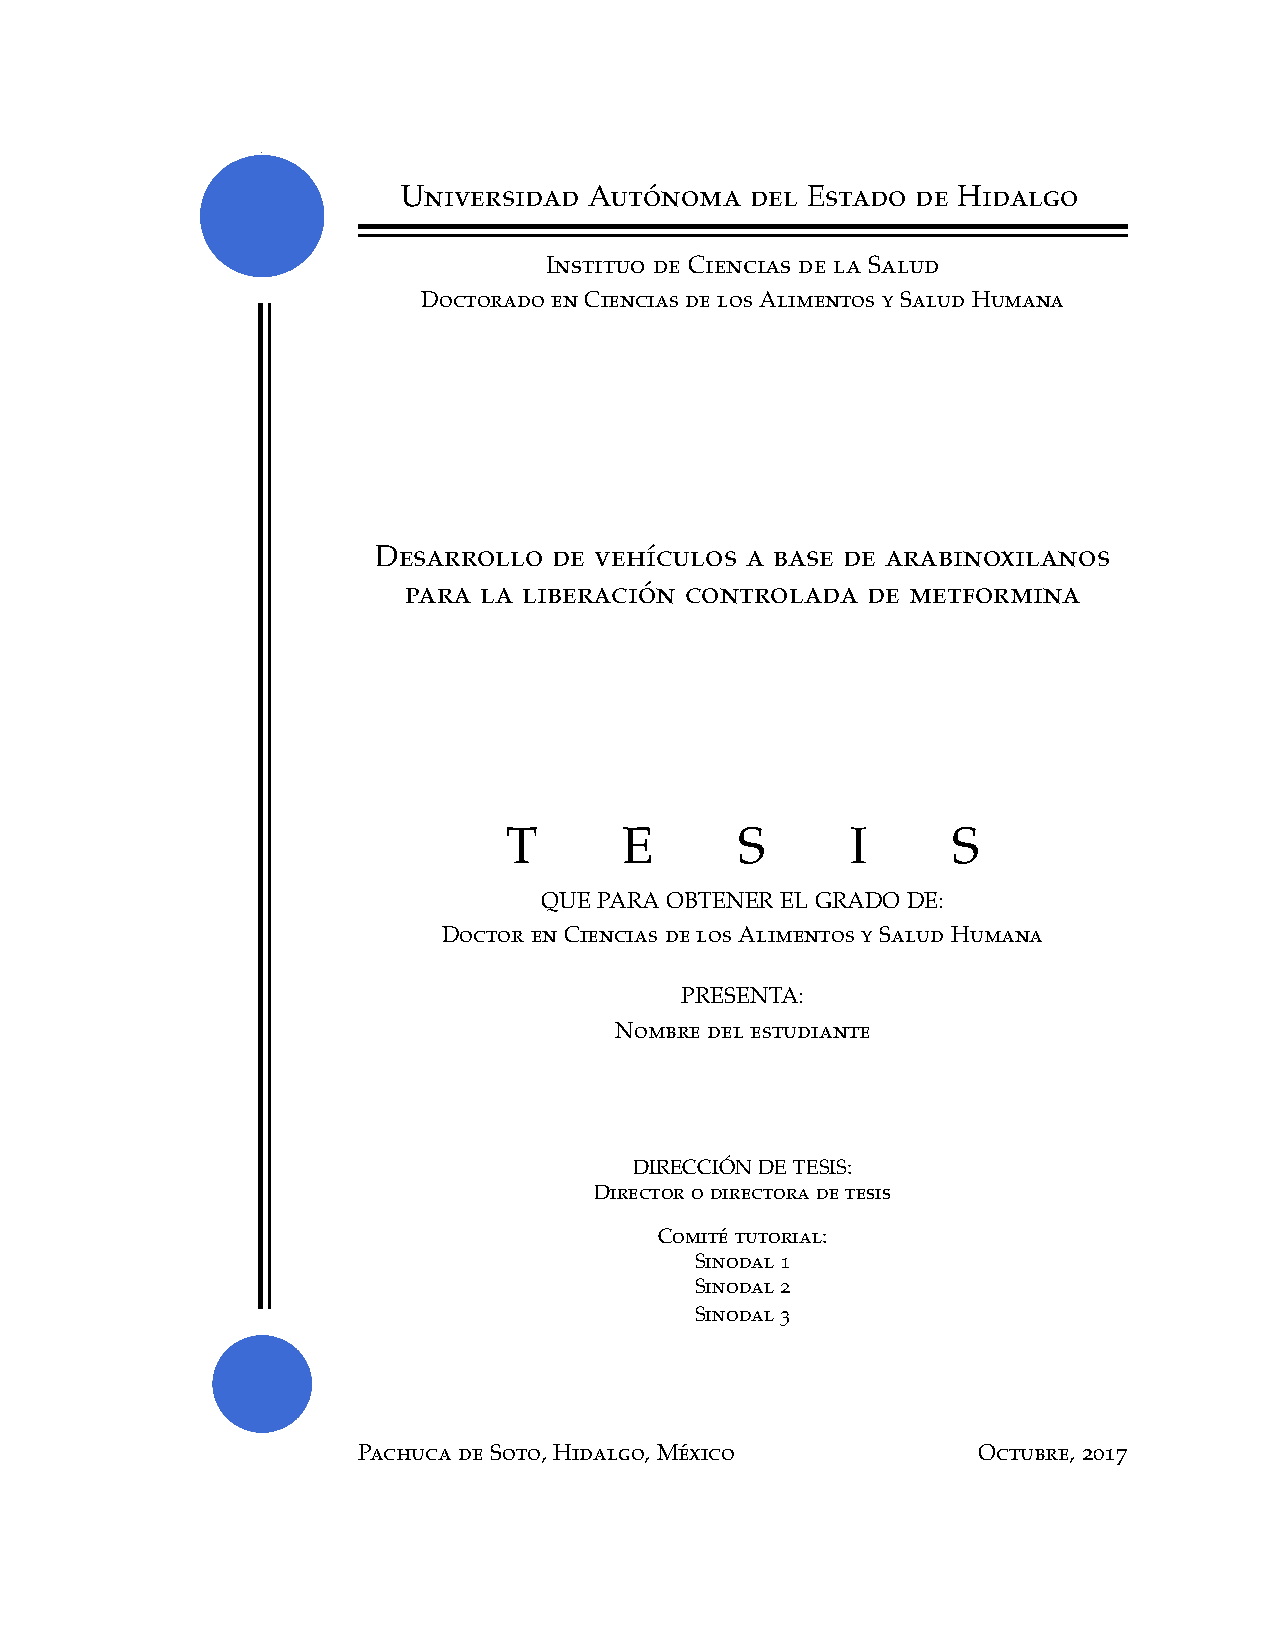
\includepdf[pages=1]{front/PortadaTesis} % Portada
	\cleardoublepage

	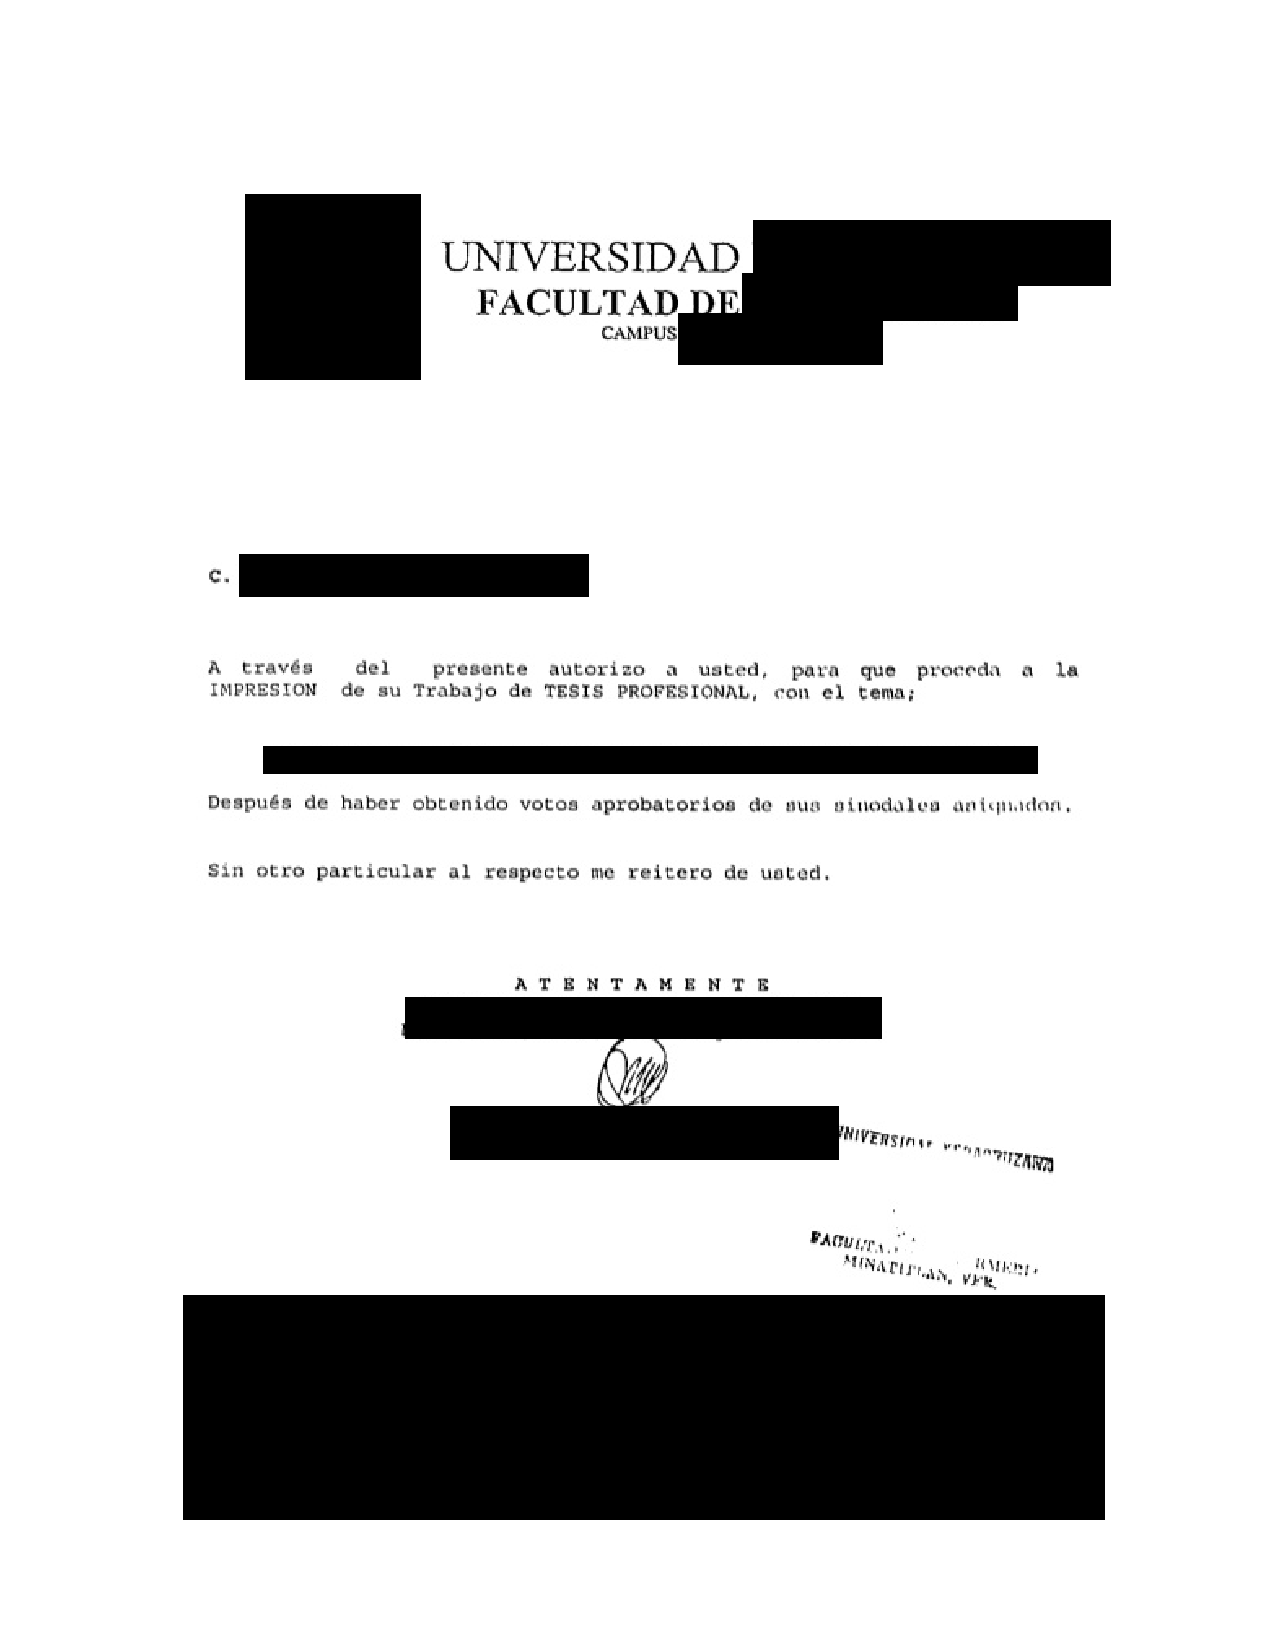
\includepdf[pages=1]{front/AutorizacionImpresion} %Autorización de impresión
	\cleardoublepage
	
	\newpage
\pagestyle{empty} % Remueve los números de página

\thispagestyle{empty}
\newenvironment{dedication} 
{\cleardoublepage
\thispagestyle{empty}
\vspace*{\stretch{1}} \begin{center} \em
} {\end{center}
\vspace*{\stretch{3}} \clearpage}
\begin{dedication}
\hfill \
\parbox{8cm}{
	\begin{verse}
	\noindent \quotefont Dedico esta plantilla en {\LaTeX} a Mayra Alejandra López Mejía, mi bonita. Esto es un testimonio de mi agradecimiento por impulsarme a crear una mejor versión de mí, por creer en mí, por tu paciencia, por tu cariño, por tu apoyo, por tu consideración, por tu resiliencia y por tu compañía. Tú me diste claridad mental, paz en mi guerra y sosiego en mi perfeccionismo. He entendido que tu posición es en el frente de batalla haciendo del mundo un lugar mejor, y la mía es contigo, por siempre a tu lado...
	\end{verse}
}
\end{dedication}

 % Dedicatoria
	\cleardoublepage
	
	\newpage
\pagestyle{empty} % Remueve los números de página

\thispagestyle{empty}

\section*{\centering \huge \it Agradecimientos}
\bigskip

\begin{enumerate}
%Incluir instutuciones educativas, gubernamentales y/o privadas que contribuyeron en el proyecto.
	\item A la Universidad Autónoma del Estado de Hidalgo...
	\item Al Centro de Investigación en Alimentación y Desarrollo A. C. ...
	\item Al Consejo Nacional de Ciencia y Tecnología...
\end{enumerate}
 % Agradecimientos
	\cleardoublepage
	
	\newpage
\pagestyle{empty} % Remueve los números de página

\vspace*{\fill}%Centra el contenido total en la hoja

\begin{center}

\begin{tikzpicture}[every node/.style={inner sep=0pt}]   
\node[text width=7cm,align=center](Text){%
\bigskip
% **************************************************
%\quotefont

Esto es un homenage a todos los idea\-lis\-tas, emprendedores, vi\-sio\-na\-rios, entusiastas y revolucionarios del mundo. Con todo mi respeto y admiración, porque ellos cambian al mundo, ellos impulsan a la humanidad hacia delante...\\
\bigskip
Mineral de la Reforma, Hgo., México a x de x del 20xx\\

\Huge
	\begin{center}
	\raisebox{-4pt}[10pt][10pt]{\textxswdown}
	\end{center}
% **************************************************
} ;
\node[shift={(-1cm,1cm)},anchor=north west](CNW)  at (Text.north west)
	             {\pgfornament[width=1cm]{61}};
\node[shift={(1cm,1cm)},anchor=north east](CNE)   at (Text.north east)
	             {\pgfornament[width=1cm,symmetry=v]{61}}; 
\node[shift={(-1cm,-1cm)},anchor=south west](CSW) at (Text.south west)
	             {\pgfornament[width=1cm,symmetry=h]{61}}; 
\node[shift={(1cm,-1cm)},anchor=south east](CSE)  at (Text.south east)   
	             {\pgfornament[width=1cm,symmetry=c]{61}};  
\pgfornamenthline{CNW}{CNE}{north}{88}
\pgfornamenthline{CSW}{CSE}{south}{88}
\pgfornamentvline{CNW}{CSW}{west}{88}
\pgfornamentvline{CNE}{CSE}{east}{88} 
\end{tikzpicture}

\end{center}

\vspace*{\fill}%Centra el contenido total en la hoja


 % OtrosAgradecimientos
	\cleardoublepage


% --- Índices, resumen y abstract
\pagestyle{fancy}
\pagenumbering{roman} % Para que inserte numeros arábigos.
\setcounter{page}{1} % Para que inicie en la página 1.

\tableofcontents
	\addcontentsline{toc}{chapter}{Índice General}
\listoffigures
	\addcontentsline{toc}{chapter}{Índice de Figuras}
\listoftables
	\addcontentsline{toc}{chapter}{Índice de Tablas}

	\phantomsection
	\renewcommand{\glossname}{Glosario} %Traducir título
	\printgloss{front/glosario} %Base de datos
			
	% **************************************************
\chapter*{Lista de Acrónimos}
\addcontentsline{toc}{chapter}{Lista de Acrónimos}
\markboth{LISTA DE ACRÓNIMOS}{LISTA DE ACRÓNIMOS}
% **************************************************

\begin{acronym}[TDMA]
% ------------- Inicia Lista -----------------------
\acro{AF}{Ácido Ferúlico}
\acro{AX}{Arabinoxilanos}
\acro{AXF}{Arabinoxilanos Ferulados}
% ------------- Termina Lista -----------------------
\end{acronym}

 % Lista de acrónimos
	% **************************************************
\chapter*{Design of devices for a controlled release from feruloylated arabinoxylans}
\addcontentsline{toc}{chapter}{Abstract} % Agregar al índice
\markboth{ABSTRACT}{ABSTRACT} % Encabezado 
% **************************************************

\begin{SummaryPhDThesis}

The aim of this investigation is to produce an encapsulant and texturizing agent from maize bran gum (MBG) for its implementation in confectionery formulations...

	\begin{HighlightsPhDThesis}
		[1] Extraction and characterization of MBG. 
		[2] Characterization of hydrogels MBG induced by laccase. 
		[3] Implementation of the MBG in confectionery.
	\end{HighlightsPhDThesis}

	\begin{keywordsPhDThesis}
		Feruloylated arabinoxylans, Hydrogels, Maize Bran Gum, Confectionery, Encapsulated.
	\end{keywordsPhDThesis}

\end{SummaryPhDThesis}
 % Abstract
	% **************************************************
\chapter*{Diseño de vehículos de liberación controlada a base de arabinoxilanos ferulados}
\addcontentsline{toc}{chapter}{Resumen} % --- Agregar al índice
\markboth{RESUMEN}{RESUMEN} % --- Encabezado 
% **************************************************

\begin{ResumenPhDThesis}

El objetivo de este trabajo fue producir un agente encapsulante y texturizante a partir de goma de pericarpio de maíz (MBG) para su implementación en productos de confitería...
	
	\begin{HighlightsPhDThesis}
		[1] Extracción y caracterización de MBG. 
		[2] Caracterización de hidrogeles de MBG. 
		[3] Implementación en productos de confitería.
	\end{HighlightsPhDThesis}

	\begin{PalabrasClavePhDThesis}
		Arabinoxilanos Ferulados, Hidrogeles, Goma de Pericarpio de Maíz, Confitería, Encapsulante.
	\end{PalabrasClavePhDThesis}

\end{ResumenPhDThesis}
 % Resumen
	% **************************************************
\chapter*{Introducción}
\addcontentsline{toc}{chapter}{Introducción} % --- Agregar al índice
\markboth{INTRODUCCIÓN}{INTRODUCCIÓN} % --- Encabezado 
% **************************************************
\chapterquote{Que lorem ipsum ad his scripta blandit partiendo, eum fastidii accumsan euripidis in, eum liber hendrerit an. Que lorem ipsum ad his scripta blandit partiendo, eum fastidii accumsan euripidis in, eum liber hendrerit an.}{Nombre del Autor}{Aportación, 2016}
% **************************************************
% --------------------------------------------------
\lettrine{D}{urante} el procesamiento de los cereales en grano, se generan subproductos de alto valor. Por ejemplo, el proceso de nixtamalización implica una hidrólisis alcalina que degrada y solubiliza los componentes de la pared celular del grano de maíz, que facilita la eliminación del pericarpio. Dicho subproducto contiene polisacáridos no celulósicos, principalmente arabinoxilanos ferulados. Otros subproductos del procesamiento de cereales tales como el pericarpio de trigo y el nejayote, se han estudiado como fuentes potenciales de arabinoxilanos ferulados, aunque se pueden extraer de otros materiales lignocelulósicos. Las caracteristicas moleculares y propiedades funcionales de los arabinoxilanos ferulados dependen de la fuente y del método de extracción de los mismos. La presencia del ácido ferúlico en esta molecula, le confiere propiedades antioxidantes y la capacidad de formar hidrogeles covalentes en presencia de agentes oxidantes, dichos hidrogeles poseen propiedades prebióticas, una estructura porosa, olor y sabor neutros, estabilidad al pH, a la temperatura y a cambios en la fuerza iónica. Se les atribuye gran potencial de aplicación como matrices para la liberación controlada de biomoléculas. Estas propiedades funcionales aumentan su potencial de aplicación en la industria agroalimentaria, biomédica y cosmética. 

El encapsulamiento implica la incorporación de aditivos en forma de cápsulas en el alimento o para enmascarar olores y sabores. Los materiales encapsulados pueden ser protegidos para aumentar su estabilidad y mantener su viabilidad. El uso de este proceso para adicionar edulcorantes tales como aspartamo y diferentes sabores en la goma de mascar, es bien conocido. Por otro lado, la industria de la confitería es una de las más competidas, por ello, el desarrollo y diversificación de productos es una estrategia para generar valor agregado y así mantenerse en el gusto de los consumidores; dicha estrategia también permite el ingreso de nuevos competidores al mercado. 

Dado de que en México, la industria productora de harina de maíz blanco, genera grandes cantidades de pericarpio, se requieren alternativas para su utilización. Por lo tanto, los arabinoxilanos ferulados extraídos de esta fuente residual, representan una excelente alternativa para el desarrollo de productos de confitería. Su extracción permitiría darles un uso como agente texturizante y emulsificante que permita obtener nuevas texturas; o como agente encapsulante para adicionar sabores, colores y/o ingredientes funcionales a las formulaciones.
 % Introducción

% **************************************************
\mainmatter % --- ContenidoPrincipal
% **************************************************
%\pagenumbering{arabic} % Para que inserte numeros arábigos.
%\setcounter{page}{1} % Para que inicie en la página 1.

	% **************************************************
\chapter{Antecedentes}
% **************************************************
\chapterquote{Que lorem ipsum ad his scripta blandit partiendo, eum fastidii accumsan euripidis in, eum liber hendrerit an. Que lorem ipsum ad his scripta blandit partiendo, eum fastidii accumsan euripidis in, eum liber hendrerit an.}{Nombre del Autor}{Aportación, 2016}
% **************************************************
% --------------------------------------------------
\section{Resumen de la investigación}
% --------------------------------------------------
\lettrine{D}{urante} el procesamiento de los cereales en grano, se generan subproductos de bajo valor agrícola, que contienen principalmente \acf{AXF}, sus características moleculares y propiedades funcionales, dependen de la fuente y del método de extracción \footnote{Ad est corrumpit.}. La presencia del \acf{AF} en la molécula, le confiere propiedades antioxidantes y la capacidad de formar hidrogeles covalentes al reaccionar con agentes oxidantes, tal como puede apreciarse en la Figura~\ref{fig:GelificacionAX}. Dichos hidrogeles de \acf{AX} poseen propiedades prebióticas, una estructura porosa, olor y sabor neutros; estabilidad al pH, a la temperatura y a cambios en la fuerza iónica \footnote{Odio omnes.}. Por lo tanto, se consideran candidatos potenciales para diseñar matrices de liberación controlada de biomoléculas \footnote{Eum hinc.}. En la Tabla~\ref{tab:Demo001} se muestran los valores obtenidos \citep{adams2003characterisation}.

\marginnote{Este es un ejemplo de nota al márgen de la página: Ut vidit lorem maiestatis his, putent mandamus gloriatur ne pro.}


\begin{figure}[h] %[htp]
    \centering 
	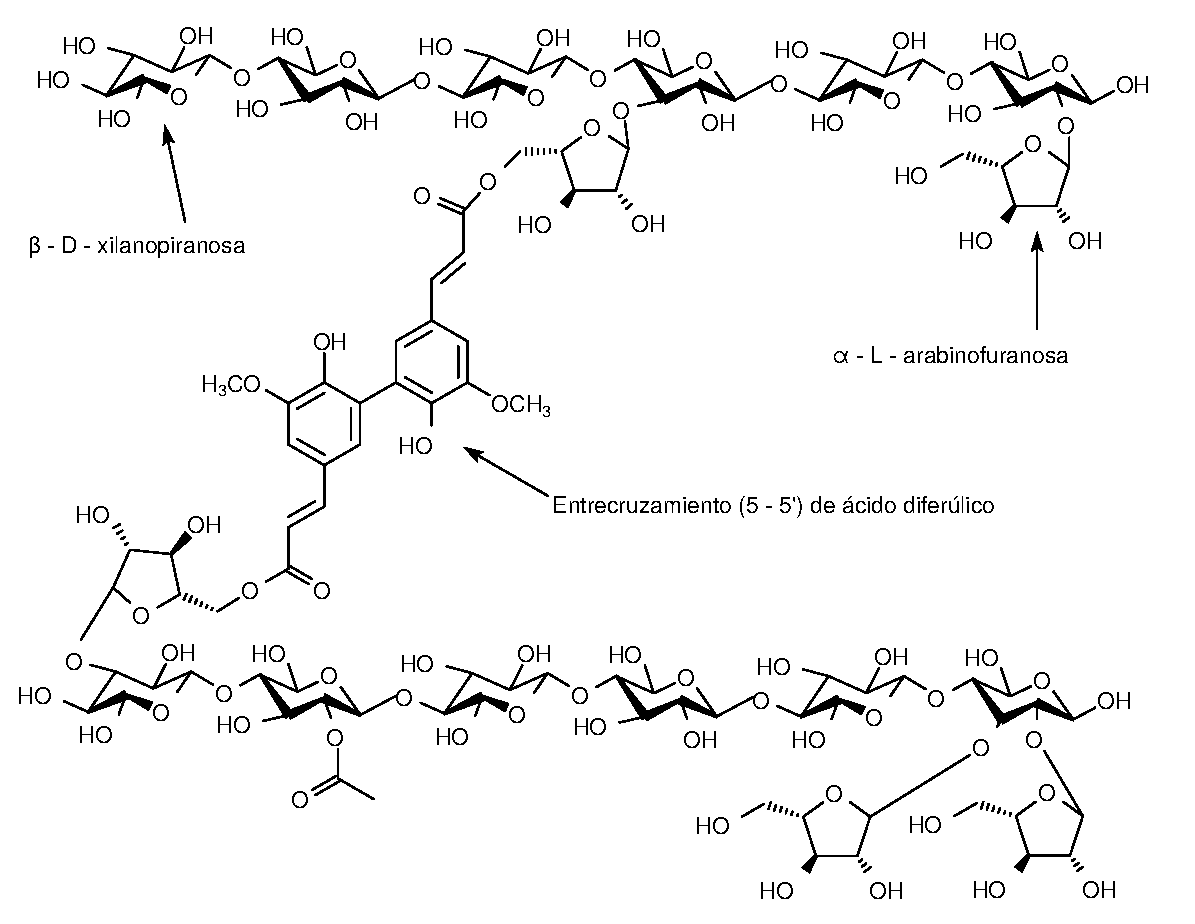
\includegraphics[width=1\linewidth]{CrossLink.pdf}
    \caption[Estructura química de hidrogeles de AX]%
    {Estructura química de hidrogeles de AX (Obtenida de \citet{andrewartha1979solution}). Oratio iriure rationibus ne his, ad est corrumpit splendide. Eum hinc argumentum te, no sit percipit adversarium, ne qui feugiat persecuti.}
    \label{fig:GelificacionAX}
\end{figure}


% --------------------------------------------------
\subsection{Eum hinc argumentum te}
% --------------------------------------------------
Estas sólo son unas pruebas de acrónimos: \ac{AX}, \acp{AX} ocurre, por defecto añade una s al final. Con \acf{AX} hacemos que aparezca el texto completo del acrónimo, con el comando \acs{AX} hacemos que aparezca la versión córta del acrónimo \footnote{Este texto es para ejemplificar.}. Primero hablaré del \gloss{CoefHuggins}. Después, haré una prueba para utilizar la \gloss{EqHuggins}. Eum hinc argumentum\index{argentum} te, no sit percipit\index{percipite} adversarium\index{adversarium}, ne qui feugiat persecuti\index{persecuti}. Odio omnes scripserit\index{scripserit} ad est, ut vidit lorem maiestatis his, putent mandamus gloriatur ne pro. Oratio\index{oratio} iriure rationibus\index{splendide!rationibus} ne his\index{splendide!Bullet Points}, ad est corrumpit splendide\index{splendide!Bullet Points}.


\begin{table}[htb]
\caption{Tabla demostrativa y notas al pie}
\begin{center}
%\begin{tabular}{ c c c c c }
% ----------------------------------------------------------
\begin{tabularx}{1\textwidth}{ l c c c c }
\toprule
\parnoteclear % tabularx will otherwise add each note thrice
\textbf{Fuente} \parnote{Los datos fueron expresados en g/100 gbs y realizados los ensayos por triplicado} & \textbf{Valor 001} & \textbf{Valor 002} & \textbf{Valor 003} & \textbf{Referencia} \\ 
\midrule
\midrule
nejayote & 5.6 & 4.7 & 6.5 & \citet{arambula2001physicochemical} \\ 
percarpio & 4.5 & 5.5 & 2.3 & \citet{azadi2013liquid} \\ 
harina & 7.8 & 3.9 & 7.4 & \citet{barron2008ftir} \\ 
\bottomrule
\end{tabularx}
% ----------------------------------------------------------
%\end{tabular}
\end{center}
\label{tab:Demo001}
\parnotes
\end{table}

 % Antecedentes
	% **************************************************
\chapter{Justificación}
% **************************************************
\chapterquote{Que lorem ipsum ad his scripta blandit partiendo, eum fastidii accumsan euripidis in, eum liber hendrerit an. Que lorem ipsum ad his scripta blandit partiendo, eum fastidii accumsan euripidis in, eum liber hendrerit an.}{Nombre del Autor}{Aportación, 2016}
% **************************************************
% --------------------------------------------------
\section{Innovación disruptiva}
% --------------------------------------------------
\lettrine{S}{oy invencible} eum hinc argumentum te, no sit percipit adversarium, ne qui feugiat persecuti. Odio omnes scripserit ad est, ut vidit lorem maiestatis his, putent mandamus gloriatur ne pro. Oratio iriure rationibus ne his, ad est corrumpit splendide. Ad duo appareat moderatius, ei falli tollit denique eos. Dicant evertitur mei in, ne his deserunt perpetua sententiae, ea sea omnes similique vituperatoribus. Ex mel errem intellegebat comprehensam, vel ad tantas antiopam delicatissimi, tota ferri affert eu nec. Legere expetenda pertinacia ne pro, et pro impetus persius assueverit.
 
 % Justificación
	% **************************************************
\chapter{Objetivos}
% **************************************************
\chapterquote{Que lorem ipsum ad his scripta blandit partiendo, eum fastidii accumsan euripidis in, eum liber hendrerit an. Que lorem ipsum ad his scripta blandit partiendo, eum fastidii accumsan euripidis in, eum liber hendrerit an.}{Nombre del Autor}{Aportación, 2016}
% **************************************************
% --------------------------------------------------
\section{Objetivo general}
% --------------------------------------------------
\lettrine{S}{oy invencible} eum hinc argumentum te, no sit percipit adversarium, ne qui feugiat persecuti. Odio omnes scripserit ad est, ut vidit lorem maiestatis his, putent mandamus gloriatur ne pro. Oratio iriure rationibus ne his, ad est corrumpit splendide.

% --------------------------------------------------
\section{Objetivos específicos}
% --------------------------------------------------
\begin{enumerate}
	\item Objetivo específico 001.
	\item Objetivo específico 002.
	\item Objetivo específico 003.
\end{enumerate}
%[label={\color{iColor002}] % Objetivos
	% **************************************************
\chapter{Materiales y métodos}
% **************************************************
\chapterquote{Que lorem ipsum ad his scripta blandit partiendo, eum fastidii accumsan euripidis in, eum liber hendrerit an. Que lorem ipsum ad his scripta blandit partiendo, eum fastidii accumsan euripidis in, eum liber hendrerit an.}{Nombre del Autor}{Aportación, 2016}
% **************************************************
% --------------------------------------------------
\section{Sección 001}
% --------------------------------------------------
\lettrine{S}{oy invencible} eum hinc argumentum te, no sit percipit adversarium, ne qui feugiat persecuti. Odio omnes scripserit ad est, ut vidit lorem maiestatis his, putent mandamus gloriatur ne pro. Oratio iriure rationibus ne his, ad est corrumpit splendide. Ad duo appareat moderatius, ei falli tollit denique eos. Dicant evertitur mei in, ne his deserunt perpetua sententiae, ea sea omnes similique vituperatoribus. Ex mel errem intellegebat comprehensam, vel ad tantas antiopam delicatissimi, tota ferri affert eu nec. Legere expetenda pertinacia ne pro, et pro impetus persius assueverit. % Metodología
	% **************************************************
\chapter{Resultados y discusión}
% **************************************************
\chapterquote{Que lorem ipsum ad his scripta blandit partiendo, eum fastidii accumsan euripidis in, eum liber hendrerit an. Que lorem ipsum ad his scripta blandit partiendo, eum fastidii accumsan euripidis in, eum liber hendrerit an.}{Nombre del Autor}{Aportación, 2016}
% **************************************************
% --------------------------------------------------
\section{Sección 001}
% --------------------------------------------------
\lettrine{S}{oy invencible} eum hinc argumentum te, no sit percipit adversarium, ne qui feugiat persecuti. Odio omnes scripserit ad est, ut vidit lorem maiestatis his, putent mandamus gloriatur ne pro. Oratio iriure rationibus ne his, ad est corrumpit splendide. Ad duo appareat moderatius, ei falli tollit denique eos. Dicant evertitur mei in, ne his deserunt perpetua sententiae, ea sea omnes similique vituperatoribus. Ex mel errem intellegebat comprehensam, vel ad tantas antiopam delicatissimi, tota ferri affert eu nec. Legere expetenda pertinacia ne pro, et pro impetus persius assueverit. % Resultados y discusión
	% **************************************************
\chapter{Conclusión}
% **************************************************
\chapterquote{Que lorem ipsum ad his scripta blandit partiendo, eum fastidii accumsan euripidis in, eum liber hendrerit an. Que lorem ipsum ad his scripta blandit partiendo, eum fastidii accumsan euripidis in, eum liber hendrerit an.}{Nombre del Autor}{Aportación, 2016}
% **************************************************
% --------------------------------------------------
\section{Sección 001}
% --------------------------------------------------
\lettrine{S}{oy invencible} eum hinc argumentum te, no sit percipit adversarium, ne qui feugiat persecuti. Odio omnes scripserit ad est, ut vidit lorem maiestatis his, putent mandamus gloriatur ne pro. Oratio iriure rationibus ne his, ad est corrumpit splendide. Ad duo appareat moderatius, ei falli tollit denique eos. Dicant evertitur mei in, ne his deserunt perpetua sententiae, ea sea omnes similique vituperatoribus. Ex mel errem intellegebat comprehensam, vel ad tantas antiopam delicatissimi, tota ferri affert eu nec. Legere expetenda pertinacia ne pro, et pro impetus persius assueverit.



 % Conclusión
	% **************************************************
\chapter{Recomendaciones}
% **************************************************
\chapterquote{Que lorem ipsum ad his scripta blandit partiendo, eum fastidii accumsan euripidis in, eum liber hendrerit an. Que lorem ipsum ad his scripta blandit partiendo, eum fastidii accumsan euripidis in, eum liber hendrerit an.}{Nombre del Autor}{Aportación, 2016}
% **************************************************
% --------------------------------------------------
\section{Sección 001}
% --------------------------------------------------
\lettrine{S}{oy invencible} eum hinc argumentum te, no sit percipit adversarium, ne qui feugiat persecuti. Odio omnes scripserit ad est, ut vidit lorem maiestatis his, putent mandamus gloriatur ne pro. Oratio iriure rationibus ne his, ad est corrumpit splendide. Ad duo appareat moderatius, ei falli tollit denique eos. Dicant evertitur mei in, ne his deserunt perpetua sententiae, ea sea omnes similique vituperatoribus. Ex mel errem intellegebat comprehensam, vel ad tantas antiopam delicatissimi, tota ferri affert eu nec. Legere expetenda pertinacia ne pro, et pro impetus persius assueverit.
 % Consideraciones futuras

%incluimos los anexos
	\renewcommand\appendixname{Anexo}
	\appendix
	% **************************************************
\chapter{Ensayos químicos}\label{anexo:CurvasCalibracion}
% **************************************************
\chapterquote{Que lorem ipsum ad his scripta blandit partiendo, eum fastidii accumsan euripidis in, eum liber hendrerit an. Que lorem ipsum ad his scripta blandit partiendo, eum fastidii accumsan euripidis in, eum liber hendrerit an.}{Nombre del Autor}{Aportación, 2016}
% **************************************************
% --------------------------------------------------
\section{Determinación de proteínas}
% --------------------------------------------------
\lettrine{S}{e} realizó mediante el Método de Bradford, para ello se mezcló una alícuota de solución de MBG al 10 \% (p/v) con 50 partes del reactivo de Bradford (previamente diluido con agua en relación 1:4). El ensayo se realizó a temperatura ambiente, el desarrollo de color se inició inmediatamente y se registró su absorbancia a 595 nm. La concentración de proteína en la muestra se determinó por interpolación utilizando una curva estándar de $\beta$-Lactoglobulina.


% --- Curvas de calibrado

% **************************************************
\backmatter % --- FinalDocumento
% **************************************************
	\phantomsection
	\addcontentsline{toc}{chapter}{Referencias}
	\renewcommand{\bibname}{Referencias}
	\bibliographystyle{back/apalike-es} %Estilo
	\bibliography{back/referencias} %Base de datos
		
	\cleardoublepage
	\phantomsection
	\addcontentsline{toc}{chapter}{Índice alfabético}
	\printindex
	
	\cleardoublepage
	\pagestyle{empty}

\hfill

\vfill


\pdfbookmark[0]{Colophon}{colophon}
\section*{Colofón}

\quotefont Tesis doctoral: Diseño de vehículos de liberación controlada a base de arabinoxilanos ferulados. Este documento fue compuesto y maquetado utilizando {\LaTeX}. Se terminó de intervenir el día XX del mes de XX del año 20XX, en Mineral de la Reforma, Hidalgo, México.

	\begin{flushright}
	\emph{
	"No es la mano de los dioses la que escribirá el final, \\
	ni el antojo del destino, ni los golpes del azar,\\
	son los actos del presente los que nos otorgarán \\
	un lugar en esta historia que jamás ha de acabar".\\
	- Hijos de la tempestad (Opera Magna)
	} \\
	%\end{flushright}
\bigskip
	%\begin{center}
	% Escribir el nombre del estudiante:
	\copyright ~ Jesús Guadalupe Pérez Flores \\
	\Huge
	\raisebox{-4pt}[10pt][10pt]{\textxswdown}
	%\end{center}
	\end{flushright}
	
\bigskip

	 
\end{document}


% Compilar con PDFLaTeX y BibTeX
% *****************************************************************
% Líneas de comandos en la terminal del editor LaTeX para compilar:
% *****************************************************************
% Glosario: bibtex Tesis.gls.aux
% Índice alfabético: makeindex -s StyleInd.ist Tesis.idx
